\documentclass[11pt]{article}

\usepackage[letterpaper,margin=0.82in,headheight=15pt]{geometry}
\usepackage[T1]{fontenc}
\usepackage[utf8]{inputenc}
\usepackage{lmodern}
\usepackage{microtype}
\usepackage{graphicx}
\usepackage{booktabs}
\usepackage{array}
\usepackage{siunitx}
\usepackage{xcolor}
\usepackage{hyperref}
\usepackage{fancyhdr}
\usepackage{titlesec}
\usepackage{caption}
\usepackage{enumitem}
\usepackage{float}

\definecolor{navy}{HTML}{17365D}
\definecolor{blue}{HTML}{2E75B6}
\definecolor{lightblue}{HTML}{D9EAF7}
\definecolor{orange}{HTML}{D55E00}
\definecolor{graytext}{HTML}{555555}

\hypersetup{
  colorlinks=true,
  linkcolor=navy,
  urlcolor=blue,
  pdftitle={Building Vibration Measurement Analysis: Turbine-Shutdown Addendum},
  pdfsubject={Paired turbine-operating and turbine-shutdown acceleration ASD comparison}
}
\graphicspath{{figures/}}
\sisetup{
  scientific-notation=true,
  round-mode=figures,
  round-precision=3,
  exponent-product=\times,
  detect-all
}
\DeclareSIUnit{\sqrthertz}{\hertz\tothe{0.5}}

\pagestyle{fancy}
\fancyhf{}
\lhead{\textcolor{graytext}{Heating-Plant Vibration Evidence}}
\rhead{\textcolor{graytext}{Physics Laboratories}}
\cfoot{\thepage}
\renewcommand{\headrulewidth}{0.4pt}

\titleformat{\section}{\Large\bfseries\color{navy}}{\thesection}{0.7em}{}
\titleformat{\subsection}{\large\bfseries\color{blue}}{\thesubsection}{0.7em}{}
\captionsetup{font=small,labelfont=bf}
\setlist{nosep,leftmargin=1.5em}
\setlength{\parindent}{0pt}
\setlength{\parskip}{0.48em}
\renewcommand{\arraystretch}{1.12}

\newcommand{\asdunit}{\si{\meter\per\second\squared\per\sqrthertz}}
% Generated by analyze_turbine_shutdown.py
\newcommand{\NumCandidateLocations}{20}
\newcommand{\NumValidPairs}{8}
\newcommand{\NumPrimaryPairs}{5}
\newcommand{\LargestPrimaryReduction}{91.5\%}
\newcommand{\SmallestPrimaryReduction}{17.2\%}
\newcommand{\LargestAllReduction}{91.5\%}
\newcommand{\SmallestAllReduction}{-9.0\%}
\newcommand{\TitanFullReduction}{37.1\%}
\newcommand{\HerzogFullReduction}{81.1\%}
\newcommand{\PhysTwoFortyFourFullReduction}{17.2\%}
\newcommand{\PipeFullReduction}{71.7\%}
\newcommand{\SidewalkFullReduction}{91.5\%}
\newcommand{\FreezerFullReduction}{-9.0\%}
\newcommand{\PipeTwentyNineDb}{-41.1}
\newcommand{\SidewalkTwentyNineDb}{-31.0}
\newcommand{\TitanTwentyNineDb}{-19.0}
\newcommand{\HerzogTwentyNineDb}{-34.4}
\newcommand{\PhysTwoFortyFourTwentyNineDb}{-10.3}


\begin{document}

\hypersetup{pageanchor=false}
\begin{titlepage}
  \centering
  \vspace*{1.2in}
  {\color{navy}\rule{\textwidth}{1.2pt}\par}
  \vspace{0.42in}
  {\Huge\bfseries Building Vibration Measurement\\[0.12in]Analysis\par}
  \vspace{0.20in}
  {\Large Turbine-Shutdown Addendum:\\[0.08in]
  Direct Confirmation of Heating-Plant Coupling\par}
  \vspace{0.42in}
  {\color{navy}\rule{\textwidth}{1.2pt}\par}
  \vfill
  \begin{tabular}{rl}
    \textbf{Evidence:} & Direct turbine-operating and shutdown comparison\\
    \textbf{Primary comparisons:} & Five paired floor and source-path locations\\
    \textbf{Physics floor pairs:} & Titan, Herzog, and PHYS 244\\
    \textbf{Report date:} & July 29, 2026\\
  \end{tabular}
  \vfill
  {\large Supplement to the Building Vibration Measurement Analysis\par}
\end{titlepage}

\hypersetup{pageanchor=true}
\pagenumbering{arabic}

\section{Direct shutdown evidence in the Physics building}

The turbine-operating spectra are shown on the left and the corresponding
shutdown spectra on the right. Every paired panel uses the same frequency
range and logarithmic amplitude scale. Paired floor spectra were
available for Titan, Herzog, and PHYS 244. PHYS 111 and PHYS 245 are omitted
because no measurement was obtained for these locations during the unscheduled shutdown.  However it should be noted from the original report that the spectrum of PHYS 245 should be comparable to PHYS 244 as before due to proximity. 

\begin{figure}[H]
\centering
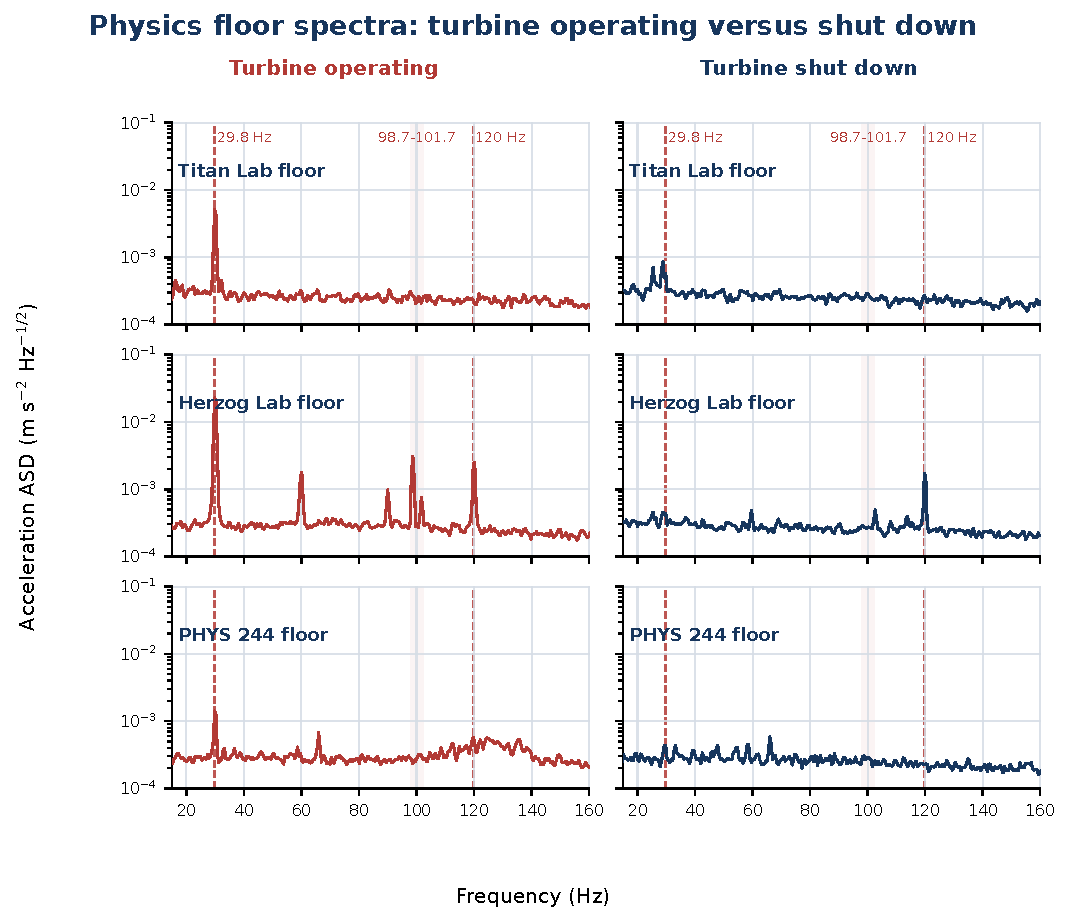
\includegraphics[width=0.93\linewidth]{laboratory_turbine_comparison.pdf}
\caption{Paired Physics floor spectra on common axes. Vertical red guides mark the 29.8 Hz line, the 98.7--101.7 Hz group, and the approximately 120 Hz line
identified in the operating-state report. The 29.8 Hz feature collapses in all three shutdown measurements. The 120 Hz peak that remains in Herzog
during shutdown is examined separately below.}
\label{fig:laboratories}
\end{figure}

At 29.8 Hz the shutdown/on ASD changes are
\TitanTwentyNineDb~dB at Titan, \HerzogTwentyNineDb~dB at Herzog, and
\PhysTwoFortyFourTwentyNineDb~dB at PHYS 244. The same line disappears from
the source-path measurements below. This is direct confirmation that the
previously observed 29.8 Hz building line was generated by the turbine.

\clearpage
\section{The source and propagation path}

The pipe and sidewalk comparison makes the source attribution decisive. The
large operating-state peaks at 29.8 Hz, 98.7--101.7 Hz, and about 120 Hz are
present at the plant and along the route toward Physics, then are absent when the turbine is shut down.

\begin{figure}[H]
\centering
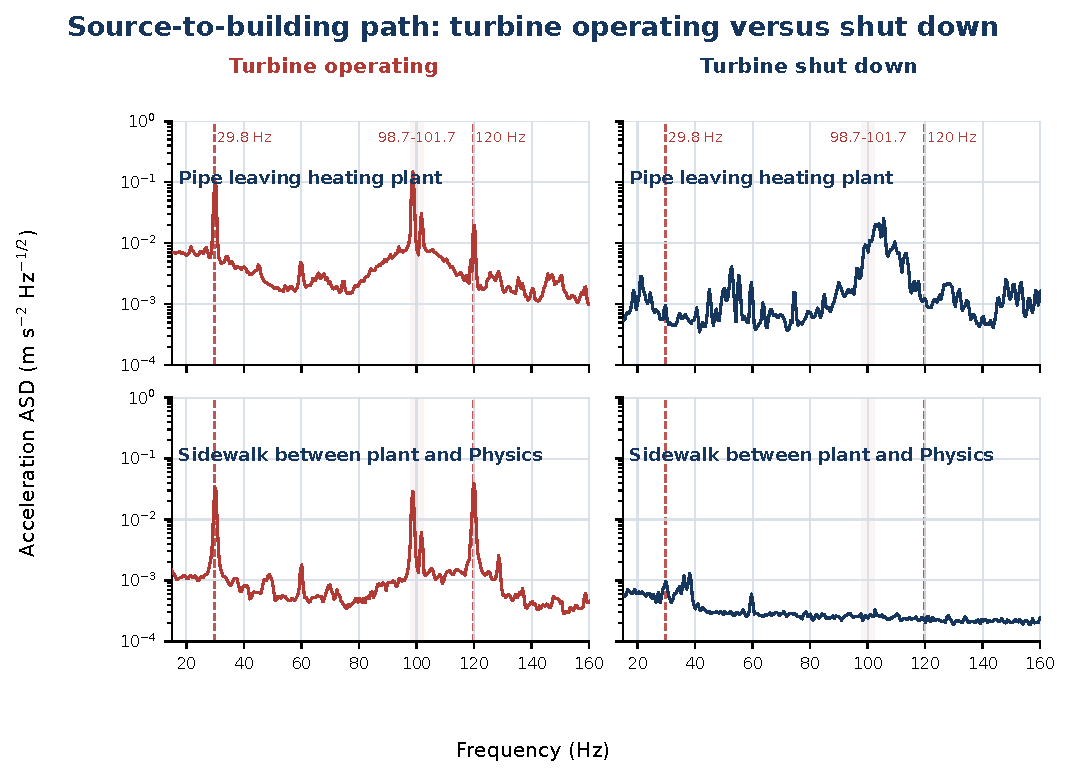
\includegraphics[width=0.93\linewidth]{source_path_turbine_comparison.pdf}
\caption{Source-path spectra with operating and shutdown states placed side
by side on identical axes. The operating-state line pattern is carried from
the plant pipe to the sidewalk. The disappearance of the external 29.8 Hz,
98.7--101.7 Hz, and 120 Hz components during shutdown
identifies them as heating-plant features.}
\label{fig:source-path}
\end{figure}

\begin{table}[H]
\centering
\caption{Primary reductions. Full-band RMS uses the same 0.5--250 Hz
definition as the main report. The last column is the shutdown/on change at
29.8 Hz; negative values are reductions.}
\label{tab:primary}
\small
\resizebox{\linewidth}{!}{\begin{tabular}{lrrrrr}
\toprule
Location & \multicolumn{2}{c}{Full-band RMS ($10^{-3}$ m s$^{-2}$)} & \multicolumn{2}{c}{Reduction (\%)} & 29.8 Hz \\
\cmidrule(lr){2-3}\cmidrule(lr){4-5}
 & On & Off & Full & 20--50 Hz & change (dB) \\
\midrule
Titan Lab floor & 6.02 & 3.79 & 37.1 & 61.6 & -19.0 \\
Herzog Lab floor & 22.3 & 4.22 & 81.1 & 91.9 & -34.4 \\
PHYS 244 floor & 4.52 & 3.75 & 17.2 & 20.5 & -10.3 \\
Pipe leaving heating plant & 176 & 49.7 & 71.7 & 94.9 & -41.1 \\
Sidewalk between plant and Physics & 59.8 & 5.08 & 91.5 & 90.1 & -31.0 \\
\bottomrule
\end{tabular}
}
\end{table}

\clearpage
\section{Turbine lines and the residual Herzog 120 Hz peak}

The shutdown test separates turbine signatures from unrelated peaks. A line
is assigned to the turbine where it is strong at the plant and sidewalk
during operation and disappears or falls sharply when the turbine stops.

\begin{table}[H]
\centering
\caption{Shutdown/on ASD change in dB at the comparison frequencies.
Negative values are reductions. The persistent Herzog value near 120 Hz is
distinguished below from the external heating-plant component.}
\label{tab:lines}
\small
\begin{tabular}{lrrrrr}
\toprule
Line (Hz) & Pipe & Sidewalk & Titan & Herzog & PHYS 244 \\
\midrule
29.8 & -41.1 & -31.0 & -19.0 & -34.4 & -10.3 \\
98.7 & -25.2 & -41.7 & -0.3 & -20.9 & 2.3 \\
101.7 & -8.5 & -27.8 & 1.1 & -9.2 & -3.6 \\
119.7 & -23.6 & -44.9 & 1.2 & -2.9 & -8.1 \\
\bottomrule
\end{tabular}

\end{table}

\textbf{The 29.8 Hz line is definitively turbine-generated:} it falls by
41.1 dB at the pipe and 31.0 dB at the sidewalk, collapsing down to the noise floor of the measurment instrument in every paired spectra. 

\textbf{The 98.7--101.7 Hz group is also a turbine source signature.} It likewise falls below the noise floor along the source path and at locations where they were prominent inside Physics.

\textbf{The external approximately 120 Hz component is turbine-related.} The 119.7 Hz amplitude falls by 23.6 dB at the pipe and effectively below the noise floor on the sidewalk adjacent to the Herzog lab, so the heating-plant contribution is no longer present. However the peak persist in the Herzog floor albeit at reduced intensity. Because 120 Hz is the common second harmonic of 60 Hz mains and can be
generated by motors and compressors, the operating ultra-cold freezer is the likely local source.

\begin{figure}[H]
\centering
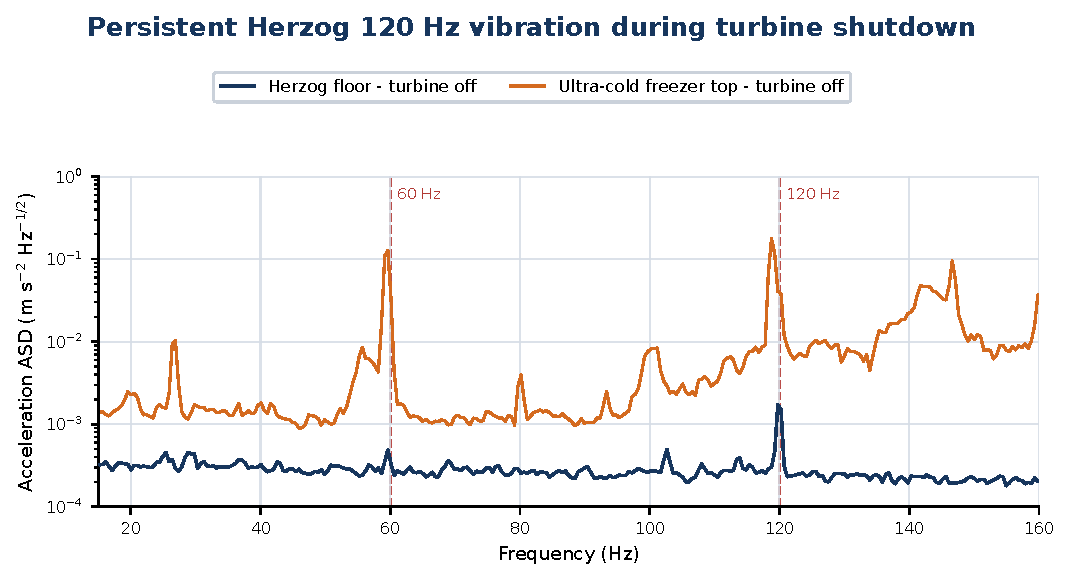
\includegraphics[width=0.82\linewidth]{herzog_freezer_shutdown_comparison.pdf}
\caption{Turbine-off spectra measured on the Herzog floor and on top of the
operating ultra-cold freezer. The external heating-plant-associated 120 Hz
component is absent in the source-path shutdown measurements, but the
persistent Herzog floor peak aligns closely with the freezer spectrum. This
makes the freezer the most likely source of the remaining laboratory
vibration near 120 Hz; a measurement with the freezer powered down is
required for definitive confirmation.}
\label{fig:freezer-herzog}
\end{figure}

\section{Conclusion}

The shutdown showed more than removal of isolated lines. Full-band RMS acceleration
falls by \PipeFullReduction\ at the plant pipe and
\SidewalkFullReduction\ on the sidewalk, while the paired room floors fall by
\TitanFullReduction\ at Titan, \HerzogFullReduction\ at Herzog, and
\PhysTwoFortyFourFullReduction\ at PHYS 244. These reductions show that the
turbine produced the clearly identified narrow lines and a substantial part
of the elevated integrated vibration background measured along the
plant-to-Physics path.

The 29.8 Hz line and 98.7--101.7 Hz source group originate with the
heating-plant turbine. The external approximately 120 Hz component is also
turbine-related, but the 120 Hz line remaining inside Herzog during shutdown
has a separate local origin. Its close frequency alignment with the operating
ultra-cold freezer makes that equipment the leading candidate, although this
attribution remains provisional until a freezer-off measurement is made.  However, as that frequency doesn't persist through the optical tables and the freezer could always be relocated, it is likely not be a question worth perusing. 


\end{document}
